\part{Diskontinuierliche Gruppen}


% ==========
\section{Möbiustransformationen}\label{sec_moebius}

\DB Es sei $X$ ein topologischer Raum und $G$ eine Gruppe von
Homöomorphismen von $X$, die effektiv operiert.
\begin{enumerate}
\item $G$ operiert \emph{diskontinuierlich}\index{diskontinuierlich}\index{Aktion!diskontinuierlich}
in $x\in X$, wenn es
eine offene Umgebung $U$ von $x$ gibt mit $g(U)\cap U=\emptyset$
für alle bis auf endlich viele $g\in G$.
\item $G$ heißt \emph{diskontinuierlich}\index{diskontinuierlich}\index{Gruppe!diskontinuierlich},
wenn es ein $x\in X$ gibt, so dass $G$ in $x$ diskontinuierlich
operiert.
\item Die Menge
\[
\Omega(G) := \{x\in X : G \text{ operiert diskontinuierlich in } x \}
\]
ist eine offene, $G$-invariante Teilmenge von $X$.
Es ist $U\subseteq \Omega(G)$.\index{$\Omega(G)$}
\end{enumerate}

\BSP Diskontinuierliche Gruppen.
\begin{enumerate}
\item Es sei $X=\hat{\CC}:=\PP^1(\CC)$ die
\emph{Riemannsche Zahlenkugel}.\index{Riemannsche Zahlenkugel}\index{$\hat{\CC}$ (Riemmansche Zahlenkugel)}
Es sei $g\in\PGL_2(\CC)$ und $G=\lag g\rag$.
\begin{enumerate}
\item $g$ ist hyperbolisch.
Dann ist $g$ konjugiert zu $z\mapsto \lambda z$ mit $\lambda\in\CC$,
$|\lambda|>1$.
Setze $U:=\{z\in\CC : 1<|z|<|\lambda| \}$.
In der folgenden Skizze ist $\lambda=\frac{5}{3}$.
\begin{center}
	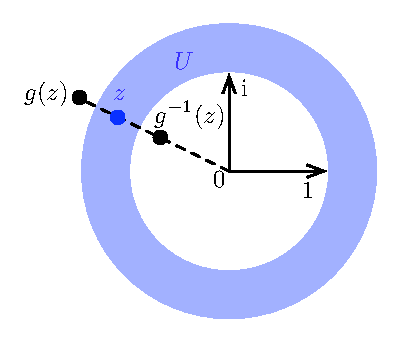
\includegraphics{grugraImages/UinC}
\end{center}
Für $z\in U$ und $n\in\ZZ$ ist $g^n(z)=\lambda^n z$,
also
\[
|g^n(z)|=|\lambda|^n |z|=
\left\{
\begin{matrix}
>|\lambda|, & n\geq 1 \\
< 1, & n\leq -1 \\
|z|, & n=0
\end{matrix}
\right..
\]
Also ist $g^n(U)\cap U=\emptyset$ für $n\neq 0$.
Damit ist $G$ diskontinuierlich und es ist
$\Omega(G)=\hat{\CC}\backslash\{0,\infty\}$.
Der Bahnenraum $\Omega(G)/G$ ist ein Torus, den man durch
Identifizieren des inneren und des äußeren Randes von $U$
erhält.
\begin{center}
	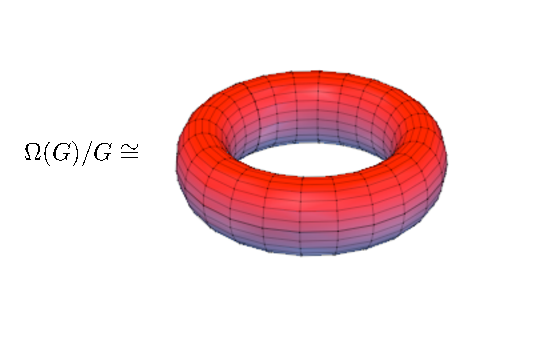
\includegraphics{Torus.pdf}
\end{center}
Die Projektion $\Omega(G)\Ra\Omega(G)/G$ ist ein
lokaler Homöomorphismus.
\item $g$ ist elliptisch.
Dann ist $g$ konjugiert zu $z\mapsto\lambda z$ mit $|\lambda|=1$.\\
Ist $\lambda$ eine $n$-te Einheitswurzel, so ist $G$ endlich und
operiert somit diskontinuierlich auf $\hat{\CC}$.
Es ist $\hat{\CC}/G\cong\hat{\CC}$.\\
Ist $\lambda$ keine Einheitswurzel, so ist $G$ unendlich und
$G\cong\ZZ$. Jeder Punkt des Einheitskreises $\{z\in\CC:|z|=1\}$
ist ein Häufungspunkt von $\{\lambda^n:n\in\ZZ\}$, denn ist
$\lambda_0$ ein Häufungspunkt, so gibt es eine Folge
$(\lambda^{n_i})_i$ mit $\lambda^{n_i}\Ra\lambda_0$,
und damit gilt auch $\lambda^{-n_{i+1}}\lambda^{n_i}\Ra 1$.
Es folgt nun, dass $G$ in keinem Punkt diskontinuierlich operiert,
da für $z\in\hat{\CC}$ die Folge $g^{-n_{i+1}}g^{n_i}(z)$ gegen
$z$ konvergiert.
\item $g$ ist parabolisch.
Dann ist $g$ konjugiert zu $z\mapsto z+1$, und $G\cong \ZZ$ ist
diskontinuierlich auf $U:=\{z\in\CC:-\frac{1}{2}<z<\frac{1}{2}\}$.
Es ist $\Omega(G)=\hat{\CC}\backslash\{\infty\}$.
Man erhält den Bahnenraum $\Omega(G)/G$, indem man die Ränder
des Streifens $U$ miteinander identifiziert und in dem so 
erhaltenen Zylinder die \glqq Ränder im Unendlichen\grqq\
miteinander identifiziert, also zu einem Punkt zusammenzieht.
\begin{center}
	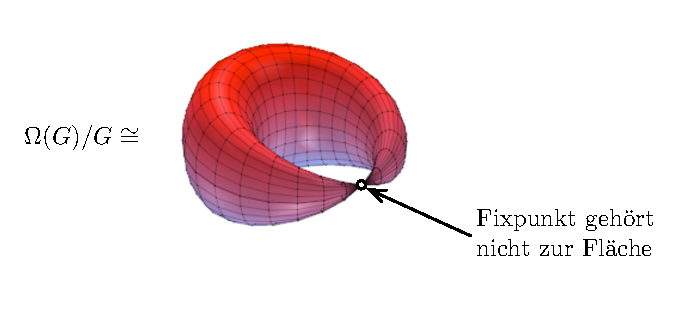
\includegraphics{cuspTorus}
\end{center}
Dieser Punkt entspricht für $z\mapsto z+1$ dem Fixpunkt $\infty$
und gehört nicht zur Fläche $\Omega(G)/G$.
Wählt man ein zu $z\mapsto z+1$ konjugiertes $g$ derart, dass
$0$ der Fixpunkt ist, so erhält man als Projektion
\[
\CC\cong \Omega(G) \Ra \Omega(G)/G\cong \CC^\times,\quad
z\mapsto \e^{2\pi\i z}.
\]
\end{enumerate}
\item Ähnlich wie für $\hat{\CC}$ können wir die Aktion von
$g\in\PGL_2(\QQ_p)$ auf $\PP^1(\QQ_p)$ betrachten.
Es sei $G=\lag g\rag$.
\begin{enumerate}
\item $g$ ist hyperbolisch. Wie im komplexen Fall ist $g$ konjugiert
zu $z\mapsto\lambda z$ mit $|\lambda|>1$, und $G$ ist diskret.
Es ist $\Omega(G)=\PP^1(\QQ_p)\backslash\{\text{Fixpunkte von }g\}$.
\item $g$ ist elliptisch. $G$ ist genau dann diskret, wenn
$g$ von endlicher Ordnung ist.
\item $g$ ist parabolisch. Dann ist $g$ konjugiert zu $z\mapsto z+1$.
Für jedes $z\in\QQ_p$ konvergiert $g^{p^n}(z)=z+p^n$ gegen $z$.
In jeder Umgebung von $z$ gibt es also unendlich viele $g^{p^n}$
und somit ist $G$ nicht diskontinuierlich.
\end{enumerate}
\end{enumerate}

\SATZ Es sei $\KK$ ein Körper der Charakteristik $0$ und
$G<\PGL_2(\KK)$ eine endliche Untergruppe.
Dann ist $G$ isomorph zu einer der folgenden Gruppen:
\begin{enumerate}
\item $\ZZ/n\ZZ$ mit $n\geq 1$.
\item $\mathrm{D}_n$ mit $n\geq 1$.
\item $\mathrm{A}_4$ (Tetraedergruppe).\index{Tetraedergruppe}
\item $\sym_4$ (Oktaedergruppe).\index{Oktaedergruppe}
\item $\mathrm{A}_5$ (Ikosaedergruppe).\index{Ikosaedergruppe}
\end{enumerate}
\bew Ohne Einschränkung nehmen wir an, dass jedes $g\in G$ zwei
Fixpunkte in $\PP^1(\KK)$ hat (notfalls müssten wir zu einer
endlichen Körpererweiterung von $\KK$ übergehen, um dies zu
gewährleisten). Es sei $n=|G|$ und $Z=\{z_1,\ldots,z_m\}$
die Menge der Fixpunkte von Elementen aus $G\backslash\{1\}$.
Dann operiert $G$ auf $Z$: Ist $z_i$ Fixpunkt von $h$, und ist
$g\in G$, so ist $g(z_i)$ ein Fixpunkt von $ghg^{-1}$.\\
Es seien nun $z_1,\ldots,z_s$ Vertreter der $G$-Bahnen.
Setze $\nu_i=|G_{z_i}|$, d.h. es ist $|G z_i|=\frac{n}{\nu_i}$
(beachte: $\nu_i|n$). Es gilt
\[
2n-2 = \SUM{s}{i=1}(\nu_i-1)\frac{n}{\nu_i},
\]
was äquivalent ist zu
\[
1\leq 2-\frac{2}{n} = \SUM{s}{i=1}\left(1-\frac{1}{\nu_i}\right)
\leq 2.
\]
Gesucht ist eine Lösung dieser Gleichung, die die Bedingungen
$n,\nu_i\in\NN$, $\nu_i\geq 2$, $\nu_i|n$ erfüllt.
Die Fälle $s=1$ und $s\geq 4$ lassen sich direkt ausschließen,
da hier die rechte Seite der Gleichung $<1$ bzw. $>2$ ist.
\begin{enumerate}
\item[]$s=2$: Es ist
$2-\frac{2}{n}=2-\frac{1}{\nu_1}-\frac{1}{\nu_2}$, und da $\nu_i|n$
gilt, folgt $\nu_1=\nu_2=n$. Somit haben alle Elemente die selben
Fixpunkte, es ist $G\cong\ZZ/n\ZZ$.
\item[]$s=3$: Ohne Einschränkung sei $\nu_1\leq\nu_2\leq\nu_3$.
Dann ist
\[
3-\frac{1}{\nu_1}-\frac{1}{\nu_2}-\frac{1}{\nu_3}=2-\frac{2}{n}
\ \lra\ 
\frac{1}{\nu_1}+\frac{1}{\nu_2}+\frac{1}{\nu_3}=1+\frac{2}{n}.
\]
Damit muss $\nu_1=2$ sein, sonst wäre die linke Seite der Gleichung
zu klein. Ebenso muss $\nu_2\leq 3$ sein.
\begin{itemize}
\item[]$\nu_2=2$: Es ist $\nu_3=\frac{n}{2}$, d.h. $G$ enthält
ein Element $\tau$ von Ordnung $\frac{n}{2}$ und ein Element
$\sigma$ von Ordnung $2$ mit $\sigma\tau\sigma=\tau^{-1}$
($\sigma$ vertauscht die Fixpunkte von $\tau$).
Es ist also $\lag\sigma,\tau\rag\cong\mathrm{D}_{\frac{n}{2}}$.
\item[] $\nu_2=3$: Es muss $\nu_3\in\{3,4,5\}$ sein.
Für $\nu_3=$ ist $G\cong\mathrm{A}_4$ und $n=12$.
Für $\nu_4=$ ist $G\cong\sym_4$ und $n=24$.
Für $\nu_5=$ ist $G\cong\mathrm{A}_5$ und $n=60$.
\qed
\end{itemize}
\end{enumerate}
